%\documentclass[ignorenonframetext, compress, 9pt, xcolor=svgnames]{beamer} 
\documentclass[notes, ignorenonframetext, compress, 10pt, xcolor=svgnames, aspectratio=169]{beamer} 
\usepackage{pgfpages}
\usepackage{pdfpages}
% These slides also contain speaker notes. You can print just the slides,
% just the notes, or both, depending on the setting below. Comment out the want
% you want.
\setbeameroption{hide notes} % Only slide
%\setbeameroption{show only notes} % Only notes
%\setbeameroption{show notes on second screen=right} % Both
\usepackage{amsmath}
\usepackage{amsfonts}
\usepackage{amssymb}
\setbeamercolor{frametitle}{fg=MidnightBlue}

\setbeamercolor{sectionpage title}{bg=MidnightBlue}
\setbeamertemplate{frametitle}[default][center]
%\setbeamertemplate{headline}{\vskip2cm}
%\setbeamertemplate{frametitle}{\color{MidnightBlue}\centering\bfseries\insertframetitle\par\vskip-6pt}
\setbeamerfont{frametitle}{series=\bfseries}
\setbeamerfont{title}{series=\bfseries}
\setbeamerfont{sectionpage}{series=\bfseries}
%\setbeamercolor{section in head/foot}{bg=MidnightBlueBlue}
%\setbeamercolor{author in head/foot}{bg=DarkBlue}
\setbeamercolor{author in head/foot}{fg=MidnightBlue}
%\setbeamercolor{title in head/foot}{bg=White}
\setbeamercolor{title in head/foot}{fg=MidnightBlue}
\setbeamercolor{title}{fg=MidnightBlue}
%\setbeamercolor{date in head/foot}{fg=Brown}
%\setbeamercolor{alerted text}{fg=DarkBlue}
%\usecolortheme[named=DarkBlue]{structure} 
%\usepackage{bbm}
%\usepackage{bbold}
\usepackage{eurosym}
\usepackage{graphicx}
%\usepackage{epstopdf}
\usepackage{hyperref}
\hypersetup{
  colorlinks   = true, %Colours links instead of ugly boxes
  urlcolor     = gray, %Colour for external hyperlinks
  linkcolor    = MidnightBlue, %Colour of internal links
  citecolor   = DarkRed %Colour of citations
}
\usepackage{multirow}
\usepackage{xspace}
\usepackage{listings}
\usepackage{natbib}
%\usepackage[sort&compress,comma,super]{natbib}
\def\newblock{} % To avoid a compilation error about a function \newblock undefined
\usepackage{bibentry}
\usepackage{booktabs}
\usepackage{dcolumn}
\usepackage[greek,frenchb]{babel}
\usepackage[babel=true,kerning=true]{microtype}
\usepackage[utf8]{inputenc}
\usepackage[T1]{fontenc}
\usepackage{natbib}
\renewcommand{\cite}{\citet}
\usepackage{longtable}
\usepackage{eso-pic}

\usepackage{xcolor}
 \colorlet{linkequation}{DarkRed} 
 \newcommand*{\SavedEqref}{}
 \let\SavedEqref\eqref 
\renewcommand*{\eqref}[1]{%
\begingroup \hypersetup{
      linkcolor=linkequation,
linkbordercolor=linkequation, }%
\SavedEqref{#1}%
 \endgroup
}

\newcommand*{\refeq}[1]{%
 \begingroup
\hypersetup{ 
linkcolor=linkequation, 
linkbordercolor=linkequation,
}%
\ref{#1}%
 \endgroup
}

\setbeamertemplate{caption}[numbered]
\setbeamertemplate{theorem}[ams style]
\setbeamertemplate{theorems}[numbered]
%\usefonttheme{serif}
%\usecolortheme{beaver}
%\usetheme{Hannover}
%\usetheme{CambridgeUS}
%\usetheme{Madrid}
%\usecolortheme{whale}
%\usetheme{Warsaw}
%\usetheme{Luebeck}
%\usetheme{Montpellier}
%\usetheme{Berlin}
%\setbeamercolor{titlelike}{parent=structure}
%\setbeamertemplate{headline}[default]
%\setbeamertemplate{footline}[default]
%\setbeamertemplate{footline}[Malmoe]
%\setbeamercovered{transparent}
%\setbeamercovered{invisible}
%\usecolortheme{crane}
%\usecolortheme{dolphin}
%\usepackage{pxfonts}
%\usepackage{isomath}
%\usepackage{mathpazo}
%\usepackage{arev} %     (Arev/Vera Sans)
%\usepackage{eulervm} %_   (Euler Math)
%\usepackage{fixmath} %  (Computer Modern)
%\usepackage{hvmath} %_   (HV-Math/Helvetica)
%\usepackage{tmmath} %_   (TM-Math/Times)
%\usepackage{tgheros}
%\usepackage{cmbright}
%\usepackage{ccfonts} \usepackage[T1]{fontenc}
%\usepackage[garamond]{mathdesign}

%\usepackage{color}
%\usepackage{ulem}

%\usepackage[math]{kurier}
%\usepackage[no-math]{fontspec}
%\setmainfont{Fontin Sans}
%\setsansfont{Fontin Sans}
%\setbeamerfont{frametitle}{size=\LARGE,series=\bfseries}
%%%add 19022021
\usepackage{enumerate}    
\usepackage{dcolumn}
\usepackage{verbatim}
\newcolumntype{d}[0]{D{.}{.}{5}}
%\setbeamertemplate{note page}{\pagecolor{yellow!5}\insertnote}
%\usetikzlibrary{positioning}
%\usetikzlibrary{snakes}
%\usetikzlibrary{calc}
%\usetikzlibrary{arrows}
%\usetikzlibrary{decorations.markings}
%\usetikzlibrary{shapes.misc}
%\usetikzlibrary{matrix,shapes,arrows,fit,tikzmark}
%%%
% suppress navigation bar
\beamertemplatenavigationsymbolsempty
%\usetheme{bunsenMod}
%\setbeamercovered{transparent}
%\setbeamertemplate{items}[circle]
%\usecolortheme[named=CadetBlue]{structure}
%\usecolortheme[RGB={225,64,5}]{structure}
%\definecolor{burntRed}{RGB}{225,64,5}
%\setbeamercolor{alerted text}{fg=burntRed} 
%\usecolortheme[RGB={0,40,110}]{structure}
%\hypersetup{linkcolor=burntRed}
%\hypersetup{urlcolor=burntRed}
%\hypersetup{filecolor=burntRed}
%\hypersetup{citecolor=burntRed}

%\usetheme{bunsenMod}
%\setbeamercovered{transparent}
%\setbeamertemplate{items}[circle]
%\usecolortheme[named=CadetBlue]{structure}
%\usecolortheme[RGB={225,64,5}]{structure}
%\definecolor{burntRed}{RGB}{225,64,5}
%\setbeamercolor{alerted text}{fg=burntRed} 
%\usecolortheme[RGB={0,40,110}]{structure}
%\hypersetup{linkcolor=burntRed}
%\hypersetup{urlcolor=burntRed}
%\hypersetup{filecolor=burntRed}
%\hypersetup{citecolor=burntRed}

%\AtBeginSection[] % Do nothing for \section*
%{ \frame{\sectionpage} }
%\setbeamertemplate{frametitle continuation}{}
\newtheorem{lemme}{Lemme}[section]
%\newtheorem{remarque}{Remarque}
\newcommand{\argmax}{\operatornamewithlimits{arg\,max}}
\newcommand{\argmin}{\operatornamewithlimits{arg\,min}}
\def\inprobLOW{\rightarrow_p}
\def\inprobHIGH{\,{\buildrel p \over \rightarrow}\,} 
\def\inprob{\,{\inprobHIGH}\,} 
\def\indist{\,{\buildrel d \over \rightarrow}\,} 
\def\sima{\,{\buildrel a \over \sim}\,} 
\def\F{\mathbb{F}}
\def\R{\mathbb{R}}
\def\N{\mathbb{N}}
\newcommand{\gmatrix}[1]{\begin{pmatrix} {#1}_{11} & \cdots &
    {#1}_{1n} \\ \vdots & \ddots & \vdots \\ {#1}_{m1} & \cdots &
    {#1}_{mn} \end{pmatrix}}
\newcommand{\iprod}[2]{\left\langle {#1} , {#2} \right\rangle}
\newcommand{\norm}[1]{\left\Vert {#1} \right\Vert}
\newcommand{\abs}[1]{\left\vert {#1} \right\vert}
\renewcommand{\det}{\mathrm{det}}
\newcommand{\rank}{\mathrm{rank}}
\newcommand{\spn}{\mathrm{span}}
\newcommand{\row}{\mathrm{Row}}
\newcommand{\col}{\mathrm{Col}}
\renewcommand{\dim}{\mathrm{dim}}
\newcommand{\prefeq}{\succeq}
\newcommand{\pref}{\succ}
\newcommand{\seq}[1]{\{{#1}_n \}_{n=1}^\infty }
\renewcommand{\to}{{\rightarrow}}
\renewcommand{\L}{{\mathcal{L}}}
\newcommand{\Er}{\mathrm{E}}
\renewcommand{\Pr}{\mathrm{P}}
%\newcommand{\Var}{\mathrm{Var}}
%\newcommand{\Cov}{\mathrm{Cov}}
%\newcommand{\corr}{\mathrm{Corr}}
%\newcommand{\Var}{\mathrm{Var}}
\newcommand{\bias}{\mathrm{Bias}}
\newcommand{\mse}{\mathrm{MSE}}
\providecommand{\Pred}{\mathcal{P}}
\providecommand{\plim}{\operatornamewithlimits{plim}}
\providecommand{\avg}{\frac{1}{n} \underset{i=1}{\overset{n}{\sum}}}
\providecommand{\sumin}{{\sum_{i=1}^n}}
\providecommand{\sumiN}{{\sum_{i=1}^N}}
\providecommand{\sumtT}{{\sum_{t=1}^T}}
\providecommand{\limp}{\overset{p}{\rightarrow}}
\providecommand{\liml}{\overset{L}{\rightarrow}}
%\providecommand{\limp}{\underset{n \rightarrow \infty}{\overset{p}{\longrightarrow}}}
%\providecommand{\limp}{\underset{n \rightarrow \infty}{\overset{p}{\longrightarrow}}}
%\providecommand{\limp}{\overset{p}{\longrightarrow}}
%\providecommand{\limd}{\underset{n \rightarrow \infty}{\overset{d}{\longrightarrow}}}
\providecommand{\limd}{\overset{d}{\rightarrow}}
\providecommand{\limps}{\overset{p.s.}{\rightarrow}}
\providecommand{\limlp}{\overset{L^p}{\rightarrow}}
\providecommand{\limprob}{\overset{p}{\underset{N\to +\infty}{\longrightarrow}}}
\providecommand{\limloi}{\overset{L}{\underset{N\to +\infty}{\longrightarrow}}}
\providecommand{\limpsure}{\overset{p.s.}{\underset{N\to +\infty}{\longrightarrow}}}
\def\independenT#1#2{\mathrel{\setbox0\hbox{$#1#2$}%
    \copy0\kern-\wd0\mkern4mu\box0}} 
\newcommand\indep{\protect\mathpalette{\protect\independenT}{\perp}}


\lstset{language=R}
\lstset{keywordstyle=\color[rgb]{0,0,1},                                        % keywords
        commentstyle=\color[rgb]{0.133,0.545,0.133},    % comments
        stringstyle=\color[rgb]{0.627,0.126,0.941}      % strings
}       
\lstset{
  showstringspaces=false,       % not emphasize spaces in strings 
  columns=fixed,
  numbersep=3mm, numbers=left, numberstyle=\tiny,       % number style
  frame=none,
  framexleftmargin=5mm, xleftmargin=5mm         % tweak margins
}
\makeatletter
%\setbeamertemplate{frametitle continuation}{\gdef\beamer@frametitle{}}
\setbeamertemplate{frametitle continuation}{\frametitle{}}
%\setbeamertemplate{frametitle continuation}{\insertcontinuationcount}
\makeatother

\theoremstyle{remark}
\newtheorem{interpretation}{Interprétation}
\newtheorem*{interpretation*}{Interprétation}

\theoremstyle{remark}
\newtheorem{remarque}{Remarque}%[section]
\newtheorem*{remarque*}{Remarque}
\usepackage[framemethod=TikZ]{mdframed} 
\usepackage{showexpl}
%\newtheorem{step}{Step}[section]
%\newtheorem{rem}{Comment}[section]
%\newtheorem{ex}{Example}[section]
%\newtheorem{hist}{History}[section]
%\newtheorem*{ex*}{Example}
%\theoremstyle{plain}
%\newtheorem{propriete}{Propri\'et\'e}
%\renewcommand{\thepropriete}{P\arabic{propriete}}
%\theoremstyle{definition}
%\newtheorem{definition}{Définition}%[section]
%\theoremstyle{remark}
%\newtheorem{exemple}{Exemple}
%\newtheorem*{exemple*}{Exemple}

\newtheorem{theoreme}{Théorème}
\newtheorem{proposition}{Proposition}
%\newtheorem{propriete}{Propri\'et\'e}
\newtheorem{corollaire}{Corollaire}
%\newtheorem{exemple}{Exemple}
%\newtheorem{assumption}{Assumption}
%\renewcommand{\theassumption}{A\arabic{assumption}}
\newtheorem{hypothese}{Hypothèse}
\renewcommand{\thehypothese}{H\arabic{hypothese}}
%\theoremstyle{definition}

%\newtheorem{definitionx}{D\'efinition}%[section]
%\newenvironment{definition}
 %{\pushQED{\qed}\renewcommand{\qedsymbol}{$\triangle$}\definitionx}
 %{\popQED\enddefinitionx}

%\newtheorem{condition}{Condition}
%\renewcommand{\thecondition}{C\arabic{condition}}
%\newcommand{\Var}{\mathbb{V}}
%\newcommand{\Var}{\mathbf{Var}}
%\newcommand{\Exp}{\mathbf{E}}
%\providecommand{\Vr}{\mathrm{Var}}
%\renewcommand{\Er}{\mathbb{E}}
%\newcommand{\LP}{\mathcal{LP}}
%\providecommand{\Id}{\mathbf{I}}
%\providecommand{\Rang}{\mathrm{Rang}}
%\providecommand{\Trace}{\mathrm{Trace}}
%\newcommand{\Cov}{\mathbf{Cov}}
%\newcommand{\Cov}{\mathbb{C}\mathrm{ov}}
\providecommand{\Id}{\mathbf{I}}
\providecommand{\Ind}{\mathbf{1}}
\providecommand{\uvec}{\mathbf{1}}
\providecommand{\vecOnes}{\mathbf{1}}
\DeclareMathOperator{\indfun}{\mathbf{1}}
\DeclareMathOperator{\Exp}{E}
\DeclareMathOperator{\Expn}{\mathbb{E}_n}
\DeclareMathOperator{\EL}{EL}
\DeclareMathOperator{\Var}{Var}
\DeclareMathOperator{\Vr}{V}
\newcommand{\boldVr}{ {\boldsymbol \Vr} }
\DeclareMathOperator{\Cov}{Cov}
\DeclareMathOperator{\corr}{corr}
\DeclareMathOperator{\perps}{\perp_s}
%\DeclareMathOperator{\Prob}{Pr}
\DeclareMathOperator{\Prob}{P}
\DeclareMathOperator{\prob}{p}
\DeclareMathOperator{\loss}{L}
\providecommand{\Corr}{\mathrm{Corr}}
\providecommand{\Diag}{\mathrm{Diag}}
\providecommand{\reg}{\mathrm{r}}
\providecommand{\Likelihood}{\mathrm{L}}
\renewcommand{\Pr}{{\mathbb{P}}}
\providecommand{\set}[1]{\left\{#1\right\}}
\providecommand{\uvec}{\mathbf{1}}
\providecommand{\Rang}{\mathrm{Rang}}
\providecommand{\Trace}{\mathrm{Trace}}
\providecommand{\Tr}{\mathrm{Tr}}
\providecommand{\CI}{\mathrm{CI}}
\providecommand{\asyvar}{\mathrm{AsyVar}}
\DeclareMathOperator{\Supp}{Supp}
\newcommand{\inputslide}[2]{{
    \usebackgroundtemplate{
     \includegraphics[page={#2},width=0.90\textwidth,keepaspectratio=true]
      %\includegraphics[page={#2},width=\paperwidth,keepaspectratio=true]
      {{#1}}}
    \frame[plain]{}
  }}
\newcommand\pperp{\perp\!\!\!\perp}
\newcommand\independent{\protect\mathpalette{\protect\independenT}{\perp}}
\def\independenT#1#2{\mathrel{\rlap{$#1#2$}\mkern2mu{#1#2}}}
\usepackage{bbm}
\providecommand{\Ind}{\mathbf{1}}
\newcommand{\sumjsi}{\underset{i<j}{{\sum}}}
\newcommand{\prodjsi}{\underset{i<j}{{\prod}}}
\newcommand{\sumisj}{\underset{j<i}{{\sum}}}
\newcommand{\prodisj}{\underset{j<i}{{\prod}}}
\newcommand{\sumobs}{\underset{i=1}{\overset{n}{\sum}}}
\newcommand{\sumi}{\underset{i=1}{\overset{n}{\sum}}}
\newcommand{\prodi}{\underset{i=1}{\overset{n}{\prod}}}
\newcommand{\prodobs}{\underset{i=1}{\overset{n}{\prod}}}
\newcommand{\simiid}{{\overset{i.i.d.}{\sim}}}
%\newcommand{\sumobs}{\sum_{i=1}^N}
%\newcommand{\prodobs}{\prod_{i=1}^N}
%\newcommand{\sumjsi}{\sum_{i<j}}
%\newcommand{\prodjsi}{\prod_{i<j}}
%\newcommand{\sumisj}{\sum_{j<i}}
%\newcommand{\prodisj}{\sum_{j<i}}

%\usepackage{appendixnumberbeamer}
\setbeamertemplate{footline}[frame number]
\setbeamertemplate{section in toc}[sections numbered]
\setbeamertemplate{subsection in toc}[subsections numbered]
\setbeamertemplate{subsubsection in toc}[subsubsections numbered]

%\makeatother
%\setbeamertemplate{footline}
%{
%    \leavevmode%
%    \hbox{%
%        \begin{beamercolorbox}[wd=.333333\paperwidth,ht=2.25ex,dp=1ex,center]{author in head/foot}%
%            \usebeamerfont{author in head/foot}\insertshortauthor
%        \end{beamercolorbox}%
%        \begin{beamercolorbox}[wd=.333333\paperwidth,ht=2.25ex,dp=1ex,center]{title in head/foot}%
%            \usebeamerfont{title in head/foot}\insertshorttitle
%        \end{beamercolorbox}%
%        \begin{beamercolorbox}[wd=.333333\paperwidth,ht=2.25ex,dp=1ex,right]{date in head/foot}%
%            \usebeamerfont{date in head/foot}\insertshortdate{}\hspace*{2em}
%            \insertframenumber{} / \inserttotalframenumber\hspace*{2ex} 
%        \end{beamercolorbox}}%
%       \vskip0pt%
 %   }
%   \makeatother
%\setbeamertemplate{navigation symbols}{}
\setbeamertemplate{itemize items}[ball]
%\setbeamertemplate{itemize items}{-}
%\newenvironment{wideitemize}{\itemize\addtolength{\itemsep}{10pt}}{\enditemize}
% \usepackage{eso-pic}
%\newcommand\AtPagemyUpperLeft[1]{\AtPageLowerLeft{%
%\put(\LenToUnit{0.9\paperwidth},\LenToUnit{0.9\paperheight}){#1}}}
%\AddToShipoutPictureFG{
%  \AtPagemyUpperLeft{{\includegraphics[width=1.1cm,keepaspectratio]{../logo-uga.png}}}
%}%
\def\figheight{3in}
\def\figwidth{4in}

%%Commands from Econometric Theory(Slides) by J. Stachurski.

\newcommand{\boldx}{ {\mathbf x} }
\newcommand{\boldu}{ {\mathbf u} }
\newcommand{\boldv}{ {\mathbf v} }
\newcommand{\boldw}{ {\mathbf w} }
\newcommand{\boldy}{ {\mathbf y} }
\newcommand{\boldb}{ {\mathbf b} }
\newcommand{\bolda}{ {\mathbf a} }
\newcommand{\boldc}{ {\mathbf c} }
\newcommand{\boldd}{ {\mathbf d} }
\newcommand{\boldi}{ {\mathbf i} }
\newcommand{\bolde}{ {\mathbf e} }
\newcommand{\boldp}{ {\mathbf p} }
\newcommand{\boldq}{ {\mathbf q} }
\newcommand{\bolds}{ {\mathbf s} }
\newcommand{\boldt}{ {\mathbf t} }
\newcommand{\boldz}{ {\mathbf z} }
\newcommand{\boldr}{ {\mathbf r} }
\newcommand{\boldm}{ {\mathbf m} }

\newcommand{\boldzero}{ {\mathbf 0} }
\newcommand{\boldone}{ {\mathbf 1} }

\newcommand{\boldalpha}{ {\boldsymbol \alpha} }
\newcommand{\boldbeta}{ {\boldsymbol \beta} }
\newcommand{\boldgamma}{ {\boldsymbol \gamma} }
\newcommand{\boldGamma}{ {\boldsymbol \Gamma} }
\newcommand{\boldtheta}{ {\boldsymbol \theta} }
\newcommand{\boldxi}{ {\boldsymbol \xi} }
\newcommand{\boldtau}{ {\boldsymbol \tau} }
\newcommand{\boldepsilon}{ {\boldsymbol \epsilon} }
\newcommand{\boldvepsilon}{ {\boldsymbol \varepsilon} }
\newcommand{\boldmu}{ {\boldsymbol \mu} }
\newcommand{\boldSigma}{ {\boldsymbol \Sigma} }
\newcommand{\boldOmega}{ {\boldsymbol \Omega} }
\newcommand{\boldPhi}{ {\boldsymbol \Phi} }
\newcommand{\boldLambda}{ {\boldsymbol \Lambda} }
\newcommand{\boldphi}{ {\boldsymbol \phi} }
\newcommand{\boldeta}{ {\boldsymbol \eta} }

\newcommand{\Sigmax}{ {\boldsymbol \Sigma_{\boldx}}}
\newcommand{\Sigmau}{ {\boldsymbol \Sigma_{\boldu}}}
\newcommand{\Sigmaxinv}{ {\boldsymbol \Sigma_{\boldx}^{-1}}}
\newcommand{\Sigmav}{ {\boldsymbol \Sigma_{\boldv \boldv}}}

\newcommand{\hboldx}{ \hat {\mathbf x} }
\newcommand{\hboldy}{ \hat {\mathbf y} }
\newcommand{\hboldb}{ \hat {\mathbf b} }
\newcommand{\hboldu}{ \hat {\mathbf u} }
\newcommand{\hboldtheta}{ \hat {\boldsymbol \theta} }
\newcommand{\hboldtau}{ \hat {\boldsymbol \tau} }
\newcommand{\hboldmu}{ \hat {\boldsymbol \mu} }
\newcommand{\hboldbeta}{ \hat {\boldsymbol \beta} }
\newcommand{\hboldgamma}{ \hat {\boldsymbol \gamma} }
\newcommand{\hboldSigma}{ \hat {\boldsymbol \Sigma} }

\newcommand{\boldA}{\mathbf A}
\newcommand{\boldB}{\mathbf B}
\newcommand{\boldC}{\mathbf C}
\newcommand{\boldD}{\mathbf D}
\newcommand{\boldI}{\mathbf I}
\newcommand{\boldL}{\mathbf L}
\newcommand{\boldM}{\mathbf M}
\newcommand{\boldP}{\mathbf P}
\newcommand{\boldQ}{\mathbf Q}
\newcommand{\boldR}{\mathbf R}
\newcommand{\boldX}{\mathbf X}
\newcommand{\boldU}{\mathbf U}
\newcommand{\boldV}{\mathbf V}
\newcommand{\boldW}{\mathbf W}
\newcommand{\boldY}{\mathbf Y}
\newcommand{\boldZ}{\mathbf Z}

\newcommand{\bSigmaX}{ {\boldsymbol \Sigma_{\hboldbeta}} }
\newcommand{\hbSigmaX}{ \mathbf{\hat \Sigma_{\hboldbeta}} }
\newcommand{\betahat}{\hat{\beta}}
\newcommand{\gammahat}{\hat{\gamma}}
\newcommand{\Uhat}{\hat{U}}
\newcommand{\Vhat}{\hat{V}}
\newcommand{\epsilonhat}{\hat{\epsilon}}
\newcommand{\sigmahat}{\hat{\sigma}}
\newcommand{\Sigmahat}{\hat{\Sigma}}
\newcommand{\Gammahat}{\hat{\Gamma}}

\newcommand{\RR}{\mathbbm R}
\newcommand{\CC}{\mathbbm C}
\newcommand{\NN}{\mathbbm N}
\newcommand{\PP}{\mathbbm P}
\newcommand{\EE}{\mathbbm E \nobreak\hspace{.1em}}
\newcommand{\EEP}{\mathbbm E_P \nobreak\hspace{.1em}}
\newcommand{\ZZ}{\mathbbm Z}
\newcommand{\QQ}{\mathbbm Q}


\newcommand{\XX}{\mathbbm X}

\newcommand{\aA}{\mathcal A}
\newcommand{\fF}{\mathscr F}
\newcommand{\bB}{\mathscr B}
\newcommand{\iI}{\mathscr I}
\newcommand{\rR}{\mathscr R}
\newcommand{\dD}{\mathcal D}
\newcommand{\lL}{\mathcal L}
\newcommand{\llL}{\mathcal{H}_{\ell}}
\newcommand{\gG}{\mathcal G}
\newcommand{\hH}{\mathcal H}
\newcommand{\nN}{\textrm{\sc n}}
\newcommand{\lN}{\textrm{\sc ln}}
\newcommand{\pP}{\mathscr P}
\newcommand{\qQ}{\mathscr Q}
\newcommand{\xX}{\mathcal X}
\newcommand{\yY}{\mathcal Y}
\newcommand{\ddD}{\mathscr D}


%\newcommand{\R}{{\texttt R}}
\newcommand{\risk}{\mathcal R}
\newcommand{\Remp}{R_{{\rm emp}}}

\newcommand*\diff{\mathop{}\!\mathrm{d}}
\newcommand{\ess}{ \textrm{{\sc ess}} }
\newcommand{\tss}{ \textrm{{\sc tss}} }
\newcommand{\rss}{ \textrm{{\sc rss}} }
\newcommand{\rssr}{ \textrm{{\sc rssr}} }
\newcommand{\ussr}{ \textrm{{\sc ussr}} }
\newcommand{\zdata}{\mathbf{z}_{\mathcal D}}
\newcommand{\Pdata}{P_{\mathcal D}}
\newcommand{\Pdatatheta}{P^{\mathcal D}_{\theta}}
\newcommand{\Zdata}{Z_{\mathcal D}}


\newcommand{\e}[1]{\mathbbm{E}[{#1}]}
\newcommand{\p}[1]{\mathbbm{P}({#1})}

% condition
\theoremstyle{definition}
\newtheorem{condition}{Condition}
\renewcommand{\thecondition}{C\arabic{condition}}
\BeforeBeginEnvironment{condition}{
  \setbeamerfont{block title}{series=\bfseries}
  \setbeamercolor{block title}{fg=MidnightBlue,bg=white}
  \setbeamercolor{block body}{fg=black, bg=gray!10}
}
\newtheorem*{condition*}{Condition}
\BeforeBeginEnvironment{condition*}{
  \setbeamerfont{block title}{series=\bfseries}
  \setbeamercolor{block title}{fg=MidnightBlue,bg=white}
  \setbeamercolor{block body}{fg=black, bg=gray!10}
}

% assumption
\theoremstyle{definition}
\newtheorem{assumption}{Assumption}
\BeforeBeginEnvironment{assumption}{
  \setbeamerfont{block title}{series=\bfseries}
  \setbeamercolor{block title}{fg=MidnightBlue,bg=white}
  \setbeamercolor{block body}{fg=black, bg=gray!10}
}
\newtheorem*{assumption*}{Assumption}
\BeforeBeginEnvironment{assumption*}{
  \setbeamerfont{block title}{series=\bfseries}
  \setbeamercolor{block title}{fg=MidnightBlue,bg=white}
  \setbeamercolor{block body}{fg=black, bg=gray!10}
}

% definition
\BeforeBeginEnvironment{definition}{
  \setbeamerfont{block title}{series=\bfseries}
  \setbeamercolor{block title}{fg=MidnightBlue,bg=white}
  \setbeamercolor{block body}{fg=black, bg=gray!10}
}
\newtheorem*{definition*}{Definition}
\BeforeBeginEnvironment{definition*}{
  \setbeamerfont{block title}{series=\bfseries}
  \setbeamercolor{block title}{fg=MidnightBlue,bg=white}
  \setbeamercolor{block body}{fg=black, bg=gray!10}
}

% theorem
\theoremstyle{plain}
\BeforeBeginEnvironment{theorem}{
  \setbeamerfont{block body}{shape=\itshape}
  \setbeamerfont{block title}{series=\bfseries}
  \setbeamercolor{block title}{fg=MidnightBlue,bg=white}
  \setbeamercolor{block body}{fg=black, bg=gray!10}
}
\newtheorem*{theorem*}{Theorem}
\BeforeBeginEnvironment{theorem*}{
  \setbeamerfont{block body }{shape=\itshape}
  \setbeamerfont{block title}{series=\bfseries}
  \setbeamercolor{block title}{fg=MidnightBlue,bg=white}
  \setbeamercolor{block body}{fg=black, bg=gray!10}
}

% definition_fr
\theoremstyle{definition}
\newtheorem{definition_fr}{Définition}%[section]
\BeforeBeginEnvironment{definition_fr}{
  \setbeamerfont{block title}{series=\bfseries}
  \setbeamercolor{block title}{fg=MidnightBlue,bg=white}
  \setbeamercolor{block body}{fg=black, bg=gray!10}
}
\newtheorem*{definition_fr*}{Définition}
\BeforeBeginEnvironment{definition_fr*}{
  \setbeamerfont{block title}{series=\bfseries}
  \setbeamercolor{block title}{fg=MidnightBlue,bg=white}
  \setbeamercolor{block body}{fg=black, bg=gray!10}
}
% theorem_fr
\newtheorem{theorem_fr}{Théorème}%[section]
\BeforeBeginEnvironment{theorem_fr}{
  \setbeamerfont{block body}{shape=\itshape}
  \setbeamerfont{block title}{series=\bfseries, shape = \upshape}
  \setbeamercolor{block title}{fg=MidnightBlue,bg=white}
  \setbeamercolor{block body}{fg=black, bg=gray!10}
}
\newtheorem*{theorem_fr*}{Théorème}
\BeforeBeginEnvironment{theorem_fr*}{
  \setbeamerfont{block body}{shape=\itshape}
  \setbeamerfont{block title}{series=\bfseries, shape = \upshape}
  \setbeamercolor{block title}{fg=MidnightBlue,bg=white}
  \setbeamercolor{block body}{fg=black, bg=gray!10}
}

% remark_fr
\theoremstyle{remark}
\newtheorem{remark_fr}{Remarque}%[section]
\BeforeBeginEnvironment{remark_fr}{
  \setbeamerfont{block title}{series=\bfseries, shape=\itshape}
  \setbeamercolor{block title}{fg=MidnightBlue,bg=white}
  \setbeamercolor{block body}{fg=black, bg=gray!10}
}
\newtheorem*{remark_fr*}{Remarque}
\BeforeBeginEnvironment{remark_fr*}{
  \setbeamerfont{block title}{series=\bfseries, shape=\itshape}
  \setbeamercolor{block title}{fg=MidnightBlue,bg=white}
  \setbeamercolor{block body}{fg=black, bg=gray!10}
}

% exemple
\theoremstyle{remark}
\newtheorem{exemple}{Exemple}%[section]
\BeforeBeginEnvironment{exemple}{
  \setbeamerfont{block title}{series=\bfseries, shape=\itshape}
  \setbeamercolor{block title}{fg=MidnightBlue,bg=white}
  \setbeamercolor{block body}{fg=black, bg=gray!10}
}
\newtheorem*{exemple*}{}
\BeforeBeginEnvironment{exemple*}{
  \setbeamerfont{block title}{series=\bfseries, shape=\itshape}
  \setbeamercolor{block title}{fg=MidnightBlue,bg=white}
  \setbeamercolor{block body}{fg=black, bg=gray!10}
}


% propriete
\theoremstyle{plain}
\newtheorem{propriete}{Propri\'et\'e}%[section]
\BeforeBeginEnvironment{propriete}{
  \setbeamerfont{block body}{shape=\itshape}
  \setbeamerfont{block title}{series=\bfseries, shape = \upshape}
  \setbeamercolor{block title}{fg=MidnightBlue,bg=white}
  \setbeamercolor{block body}{fg=black, bg=gray!10}
}
\newtheorem*{propriete*}{Propri\'et\'e}
\BeforeBeginEnvironment{propriete*}{
  \setbeamerfont{block body}{shape=\itshape}
  \setbeamerfont{block title}{series=\bfseries, shape = \upshape}
  \setbeamercolor{block title}{fg=MidnightBlue,bg=white}
  \setbeamercolor{block body}{fg=black, bg=gray!10}
}


% remark
\theoremstyle{remark}
\newtheorem{remark}{Remark}%[section]
\BeforeBeginEnvironment{remark}{
  \setbeamerfont{block body}{shape=\itshape}
  \setbeamerfont{block title}{series=\bfseries}
  \setbeamercolor{block title}{fg=MidnightBlue,bg=white}
  \setbeamercolor{block body}{fg=black, bg=gray!10}
}
\newtheorem*{remark*}{Remark}
\BeforeBeginEnvironment{remark*}{
  \setbeamerfont{block body }{shape=\itshape}
  \setbeamerfont{block title}{series=\bfseries}
  \setbeamercolor{block title}{fg=MidnightBlue,bg=white}
  \setbeamercolor{block body}{fg=black, bg=gray!10}
}


\usepackage{color}
\usepackage{tikz}
\usetikzlibrary{positioning}
\usepackage{enumerate}   
\usepackage{multirow}
%\setbeamersize{text margin left=1.5em,text margin right=1.5em} 
%\setbeamersize{text margin left=1.2cm,text margin right=1.2cm} 
\setbeamersize{text margin left=1.5em,text margin right=1.5em} 
%\usepackage{xr}
%\externaldocument{Econometrie1_UGA_P2e}
  \usepackage{eso-pic}
%\newcommand\AtPagemyUpperLeft[1]{\AtPageLowerLeft{%
%\put(\LenToUnit{0.9\paperwidth},\LenToUnit{0.85\paperheight}){#1}}}
%\AddToShipoutPictureFG{
 % \AtPagemyUpperLeft{{\includegraphics[width=1.1cm,keepaspectratio]{logoUGA2020.pdf}}}
%}%

%\setbeamercolor{title}{fg=black}
%\setbeamercolor{frametitle}{fg=black}
%\setbeamercolor{section in head/foot}{fg=black}
%\setbeamercolor{author in head/foot}{bg=Brown}
%\setbeamercolor{date in head/foot}{fg=Brown}
\setbeamertemplate{section page}
{
    \begin{centering}
    \begin{beamercolorbox}[sep=11pt,center]{part title}
    \usebeamerfont{section title}\thesection.~\insertsection\par
    \end{beamercolorbox}
    \end{centering}
}
%\titlegraphic{\includegraphics[width=1cm]{logoUGA2020.pdf}}
\title[]{ \textbf{Économie Industrielle}\footnote{responsable du cours: Sylvain Rossiaud} \\ (UGA, L3 Éco, S2) \\ }
\subtitle{Travaux dirigés: TD1-TD3\\ 
(éléments de correction sur les commentaires de textes)}
\date{\today}
\author{Michal W. Urdanivia\inst{*}}
\institute{\inst{*}UGA, Facult\'e d'\'Economie, GAEL, \\
e-mail:
 \href{
     mailto:michal.wong-urdanivia@univ-grenoble-alpes.fr}{michal.wong-urdanivia@univ-grenoble-alpes.fr}}

%\titlegraphic{\includegraphics[width=1cm]{logoUGA2020.pdf}
%}

\begin{document}

%%% TIKZ STUFF
\usetikzlibrary{positioning}
\usetikzlibrary{snakes}
\usetikzlibrary{calc}
\usetikzlibrary{arrows}
\usetikzlibrary{decorations.markings}
\usetikzlibrary{shapes.misc}
\usetikzlibrary{matrix,shapes,arrows,fit,tikzmark}
\usetikzlibrary{shapes}
\tikzset{   
        every picture/.style={remember picture,baseline},
        every node/.style={anchor=base,align=center,outer sep=1.5pt},
        every path/.style={thick},
        }
\newcommand\marktopleft[1]{
    \tikz[overlay,remember picture] 
        \node (marker-#1-a) at (-.3em,.3em) {};%
}
\newcommand\markbottomright[2]{%
    \tikz[overlay,remember picture] 
        \node (marker-#1-b) at (0em,0em) {};%
}
\tikzstyle{every picture}+=[remember picture] 
\tikzstyle{mybox} =[draw=black, very thick, rectangle, inner sep=10pt, inner ysep=20pt]
\tikzstyle{fancytitle} =[draw=black,fill=red, text=white]
\tikzstyle{observed}=[draw,circle,fill=gray!50]



\begin{frame}
\titlepage
\end{frame}
\begin{frame}
 \tableofcontents
    \end{frame}
%\begin{frame}
%\frametitle{Contenu}
%\tableofcontents[pausesections, pausesubsections]
%\end{frame}

%\section{Qu'est-ce que l’économétrie ? A quoi (à qui) ça sert ?}
%\frame{\sectionpage}
%\begin{frame}
%  \tableofcontents  
%\end{frame}


\section{TD1: \cite{ArquieBertin2020}}
\frame{\sectionpage}
\begin{frame}[allowframebreaks]{(a) Marché pertinent}
\begin{itemize}
\item Vous pouvez consulter ici: 
    \url{https://www.concurrences.com/fr/dictionnaire/marche-pertinent}. 
\item Un \textbf{\underline{marché de produits en cause}} comprend tous les produits et/ou services 
que le consommateur considère comme interchangeables ou substituables 
en raison de leurs caractéristiques, de leur prix et de l’usage auxquels ils sont destinés.
\item Le \textbf{\underline{marché pertinent géographique}} comprend 
le territoire sur lequel les entreprises concernées concourent à l’offre et à 
la demande des produits ou services en cause, sur lequel les conditions de concurrence 
sont suffisamment homogènes.

\framebreak

\item Points sur lesquelles insister: 
\begin{enumerate}[-]
\item double dimension d’un marché pertinent: produit et géographique,
\item calcul des élasticités-prix croisée,
\item importance de ce concept pour l’ensemble des études de cas qui seront étudiées 
par la suite concernant les stratégies de recherche de pouvoir de marché de la part des firmes. 
\end{enumerate}
\end{itemize}
\end{frame}

\begin{frame}[allowframebreaks]{(b) Paradigme S-C-P et concentration}
\begin{itemize}
   \item \underline{\textbf{Objectif}}: retour sur la construction et la 
   lecture structuraliste du paradigme 
   \href{https://fr.wikipedia.org/wiki/Structure\_comportement\_performance}{SCP} en 
   éco industrielle\footnote{Vous pouvez consulter ici aussi: 
   \url{http://www.analyse-sectorielle.fr/2011/11/objectif-dune-analyse-sectorielle/}}. 
   \item \textbf{\underline{Rappel}}: 
   \begin{enumerate}[-]
    \item Grille d’analyse sectorielle développée par l’école de Harvard pour qui 
    l’éco indus doit s’attacher à étudier l’impact des structures de marché sur 
    le comportement des entreprises. 
    \item Les principaux auteurs en sont 
    \href{https://fr.wikipedia.org/wiki/Edward\_Mason}{Edward Mason (1899-1992)}
    et \href{https://fr.wikipedia.org/wiki/Joe\_Bain}{Joe Bain (1912-1981)}. 

    \framebreak

    \item L’enchaînement analytique du paradigme S-C-P est donc: 
    \begin{enumerate}[(i)]
    \item l’étude des structures de marché, 
    \item analyse des comportements des entreprises, 
    \item des performances réalisées. 
    \end{enumerate}
    \item Les performances sont donc supposées dépendre des stratégies des firmes 
    qui elles-mêmes dépendent de la structure du marché, 
    en particulier du degré de concentration des entreprises. 
    \item Par exemple, les profits élevés (performance), supposent 
    une collision entre les firmes en matière de prix (stratégie) elle-même permise 
    par une forte concentration dans la branche (structure). 

    \framebreak 

    \item La lecture structuraliste se réalise de manière descendante et unidirectionnelle. 
    \vspace{0.5cm}

    \begin{figure}[h]
    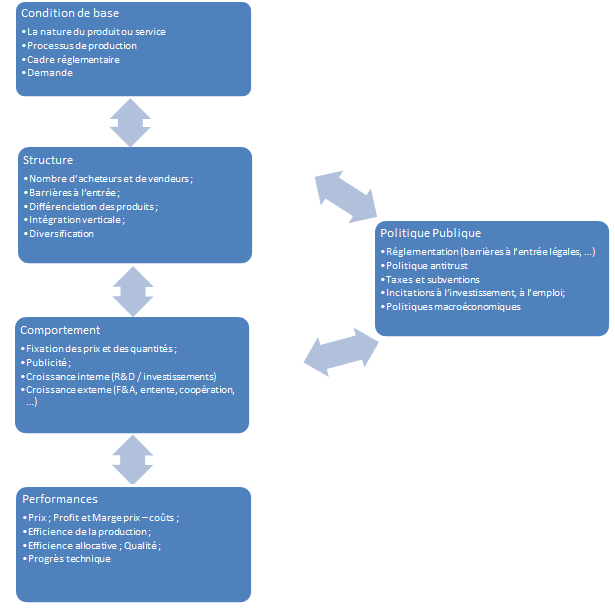
\includegraphics[width=5cm]{Analyse-Sectorielle-Modele-SCP.png}
    \caption{Explication technologique de la concentration au prisme du paradigme SCP
    \protect\linebreak
        Source: \url{http://www.analyse-sectorielle.fr/2011/11/objectif-dune-analyse-sectorielle/}}
    \end{figure}
   \end{enumerate}
\end{itemize}
\end{frame}

\begin{frame}[allowframebreaks]{(c) Harvard vs. Chicago}
\begin{itemize}
\item \textbf{\underline{Harvard:}}
\begin{enumerate}[-]
    \item Idée d’une "concentration néfaste".
    \item La corrélation positive qui existe habituellement entre degré de concentration et taux de profit 
    élevé tient aux comportements anti-concurrentiels des entreprises (= hypothèse de la collusion). 
    \item De ce point de vue, \textbf{la politique de la concurrence doit être pro-active}: 
    \begin{enumerate}[$\star$]
    \item Les autorités de la concurrence doivent contrôler, voire sanctionner les comportements des firmes susceptibles 
    de créer des positions dominantes sur les marchés qui, compte tenu des conditions de base, 
    en auraient été autrement dépourvus
    \end{enumerate}
    \item Ce faisant, l’objectif est de maintenir les conditions d’une "concurrence praticable", 
    c’est-à-dire une structure d’organisation dans laquelle les tendances à la concurrence 
    sont plus fortes que les tendances à la collusion.
\end{enumerate}
\framebreak
\item \textbf{\underline{Chicago:}}
\begin{enumerate}[-]
\item L'idée des "super-stars" développée (et critiquée) dans le texte fait écho 
au travail de l'école 
de Chicago durant les années 1970, de Harold Demsetz en particulier:
\begin{enumerate}[$\star$]
    \item Cet auteur conteste la relation causale établie par les économistes de Harvard entre taux de concentration élevé et taux de rentabilité supranormal.
    \item Surtout, si cette corrélation positive existe, il faut y voir le résultat de l’efficacité productive des grandes firmes et non pas le résultat de comportements anti-concurrentiels.
    \item Il s’agit de "l’hypothèse de l’efficacité" développée par Harold Demsetz pour s’opposer à "l’hypothèse de la collusion " 
    mise en avant par les auteurs de Harvard.
    \item Pour Chicago, les plus grandes firmes évoluant sur un marché concentré sont 
    donc fondamentalement plus productives.
\end{enumerate}
\item En outre, les auteurs de l’école de Chicago mettent en évidence que la structure (degré de concentration)
 doit elle-même être considérée comme le résultat des performances des firmes;
 \item les positions dominantes que certaines firmes peuvent acquérir 
 tiennent à leur efficacité productive supérieure. 
 \item Ces positions dominantes ne peuvent néanmoins être que temporaires puisque sous la pression 
 concurrentielle le surprofit entraînera l’entrée de nouvelles firmes sur le marché. 
%(voir par exemple 
 %\cite{DemsetzJLE1973}, ou \cite{AlchianDemsetzAER1972}).
\end{enumerate}
\end{itemize}
\end{frame}

\begin{frame}[allowframebreaks]{(d) Microsoft(Procés)}
\begin{itemize}
\item \textbf{\underline{Objectif}}: 
\begin{enumerate}[-]
\item revenir sur école de Chicago/théorie du marché contestable dont on retrouve 
ici certaines idées fondamentales. 
\item Ces idées justifient une approche plus libérale - ou moins interventionniste - de la part 
des autorités de la concurrence, comparativement à l’école de Harvard. 
\item Pour Chicago/théorie du marché contestable:
\begin{enumerate}[(i)]
\item La concentration industrielle n’est a priori pas inquiétante. 
Les grandes firmes ont atteint leurs tailles parce qu’elles sont, avant tout, les plus productives. 
\item Le nombre de firmes présentes sur un marché ainsi qu’une répartition inégalitaire des 
parts de marché ne sont pas de bons indicateurs de l’intensité de la concurrence. La concurrence 
potentielle-contestabilité du marché permet de conduire à des performances 
proches de l’idéal poursuivi par la théorie concurrentielle. 
(cf. Théorie du marché contestable).
\item Vision dynamique du processus concurrentiel. Le monde industriel est en perpétuel 
mouvement, et les positions dominantes sont donc par essence temporaires. 
\end{enumerate}
\end{enumerate}  
\end{itemize}
\end{frame}

\section{TD2:  Transdev Group versus SNCF (Ouibus)}
\frame{\sectionpage}
\begin{frame}[allowframebreaks]{(1) Politique de prix de prédation}
\begin{itemize}
\item \textbf{\underline{Rappel(c.f. CM)}}:

\medskip

"La prédation est une pratique tarifaire consistant, pour un opérateur dominant, à vendre en dessous de ses coûts de production dans le but d’éliminer, d’affaiblir ou de discipliner ses concurrents sous réserve de la possibilité de récupérer
 à terme et sous quelque forme que ce soit les pertes accumulées délibérément"\\
 (Autorité de la concurrence, affaire Wanadoo, 2002)

 \item Points à souligner: 
 \begin{enumerate}[-]
\item arbitrage temporel: 
\begin{enumerate}[$\star$]
    \item cette stratégie n’est rationnelle/rentable que si les pertes qu’elle subit dans un premier temps pour éliminer ses concurrents présents ou potentiels sont compensées par les gains futurs
\end{enumerate} 
\item Pratique sanctionnée
\begin{enumerate}[$\star$]
    \item raison: prix prédateur est guidé par l’intention 
    d’exclure du marché un ou des concurrents par des moyens autres que le processus concurrentiel "normal" / par le "mérite".
\end{enumerate} 
 \end{enumerate}
\end{itemize}
\end{frame} 
\begin{frame}[allowframebreaks]{(2) Argumentaire de l'autorité de la concurrence}
\begin{itemize}
\item 4 éléments à prendre en compte: 
\begin{enumerate}
    \item \textbf{Définition du marché en cause/marché pertinent}: RAS
    \item \textbf{Rôle des subventions croisées} :
    \begin{enumerate}[$\star$]
        \item permettent – selon transdev – à la SNCF de soutenir les prix bas. 
        \item il a été développé en CM la problématique et le débat relatif au manque de crédibilité des politiques de prix de prédation.
        \item dans le cas analysé, Transdev considère que  ce sont les subventions croisées qui permettent d’assurer la crédibilité des prix prédateurs. 
    \end{enumerate}
    \item \textbf{Test de coûts et délimitation entre les 3 zones.}
    \begin{enumerate}[$\star$]
        \item Ces trois zones ont été présentées en CM (p. 22).
        \item Il convient donc peut-être d’insister sur les spécificités du "marché émergent"  
        mises en évidence dans l’analyse de l’autorité de la concurrence et qui expliquent 
        selon elle que les prix se situent dans la zone grise:

        \medskip

        "ce qui anime l’entreprise est davantage une logique de retour sur investissement
         à horizon raisonnable qu’une logique de couverture immédiate des coûts."
    \end{enumerate}
    \item Absence d’éléments permettant de considérer que les "tarifs agressifs" 
    de Ouibus constituent une pratique de prédation ou sont fixéx dans 
    le cadre d’un plan ayant pour but d’éliminer un ou des concurrences 
    ni qu’ils sont susceptibles de provoquer des effets, potentiels ou reels, d’éviction (p. 30).  
\end{enumerate}
\end{itemize}
\end{frame}

\section{TD3: \cite{CombeMonierREF2012} }
\frame{\sectionpage}

\begin{frame}[allowframebreaks]{Question: Concentration}
    \begin{itemize}
        \item Un petit nombre d’offreurs.
        \begin{enumerate}[-]
\item Facilité pour négocier un accord. (faible coût de
transactions)
\item Un + grand nombre -> hausse du coût de détection d’un
tricheur.
\item Conséquence: incitation à forcer les concurrents à sortir du marché.
        \end{enumerate}
        \item Échantillon de 87 cartels détectés au cours de la période 67-2007.
        \begin{enumerate}[-]
        \item nombre moyen de participant : 8.
        \item La durée de vie et le pouvoir de marché d’un cartel est
        positivement corrélé à la concentration du secteur.
    \end{enumerate}
    \end{itemize}
\end{frame}

\begin{frame}[allowframebreaks]{Question : Caractéristiques principales}
    \begin{itemize}
        \item Faible élasticité-prix de la D.
        \begin{enumerate}[-]
        \item Fort pouvoir de marché.
        \item Une baisse (ou une hause) des prix ne va pas
        sensiblement changer la demande.
        \end{enumerate}
        \item Homogénéité des produits et des coûts
        \begin{enumerate}[-]
        \item Pas de stratégie de différenciation possible.
        \item L’hétérogénéité des biens, en réduisant la transparence du
        marché et donc la capacité à punir rapidement les tricheurs
        rend la collusion plus ardue.
        \item Des coûts symétriques facilite également l’entente (Pas
        d’asymétrie d’information->transparence + partage du marché facilité)
       \end{enumerate}
       \item L’existence d’obstacles à l’entrée et à la sortie (de nature juridique et éco) 
       constitue une condition favorable à l’apparition d’un cartel.
       \begin{enumerate}[-]
       \item +Mise en place de BE stratégique possibles.
       \item Si non existence-> entrée de concurrents potentiels.
    \end{enumerate}
    \item Ainsi, dans la plupart des cas, les entreprises incriminées opèrent pour
     l’essentiel sur des marchés de biens intermédiaires.
     \begin{enumerate}[-]
    \item la vente de détail et les services aux conso sont en effet peu représentés (à l’exception des services financiers).
    \item En outre, de nombreux cartels affectent des industries pour lesquelles les BE sont significatives (ind chimique).
    \item L’élasticité-prix de la D faible (ce qui est le cas généralement pour les produits intermédiaires).
     \end{enumerate}
    \item • Les résultats sont donc relativement conformes aux conclusions de la th. éco. selon laquelle la collusion est d’autant 
    plus probable que les produits sont homogènes, les BE fortes et l’élasticité-prix de la D faible.
    \end{itemize}
\end{frame}
   
\begin{frame}[allowframebreaks]{References}
\bibliographystyle{jpe}
\bibliography{../Biblio}
\end{frame}

\end{document}
